\documentclass[10pt,pdf,russian]{beamer}
\usetheme{Warsaw}
%\usertheme{Singapur}
%\title{Когда не выполнен закон нуля и единицы?}
%\aythor{Медведева Анна}
\usepackage[utf8]{inputenc}
\usepackage[russian]{babel}
\usepackage{graphics}


\begin{document}

\title{Модификация модели глубокого обучения по ковариационной матрице параметров.}
\author{Иванов И.С.}
\institute{Московский Физико-Технический Институт}
\date{Долгопрудный, 2015}

\begin{frame}
	\titlepage
\end{frame}

\begin{frame}
\begin{block}{Цель исследования}
Предложить эффективный способ модификации модели глубокого обучения в задаче классификации временных рядов, основываясь на анализе ковариационной матрицы параметров модели.
\end{block}

\begin{block}{Подходы}
Модифицированный метод Белсли анализа мультиколлинеарности
\end{block}


\begin{block}{Проблемы}
Большой размер матрицы ковариаций параметров модели
\end{block}
\end{frame}

\begin{frame}{Список литературы}
\begin{enumerate}

\bibitem{pop-choose}Попова М., Стрижов В.: Выбор оптимальной модели классификации физической активности по измерениям акселерометра .

\bibitem{pop-build}Попова М., Стрижов В.: Построение сетей глубокого обучения для классификации временных рядов.

\end{enumerate}
\end{frame}

\begin{frame}{Постановка задачи}
\begin{itemize}
\item $\mathfrak{D} =\left\{ (\mathbf{x}_i, \mathbf{t}_i) \right\}$ - выборка.
\item $\mathbf{f} : (\mathbf{w},\mathbf{X}) \mapsto \mathbf{y}$ - модель классификации, где $\mathbf{w} = [w_1, \dots,w_j,\dots,w_k]^{\T}$ - вектор параметров модели, $\mathbf{X} \in \mathbb{R}^{n\times m}$ - матрица плана, $\mathbf{y} \in \{0,1\}^z$ - зависимая переменная. 
\item В данной работе в качестве базовой модели рассматривается суперпозиция автокодировщиков и двухслойных нейронных сети.
\end{itemize}
Требуется: модифицировать модель, согласно критериям устойчивости и точности.
\end{frame}

\begin{frame}{Цели эксперимента}
\begin{itemize}
\item Сравнить влияние различных методов модификации пространства параметров модели в процессе обучения на её качество.
\item Выбрать оптимальный метод модификации.
\end{itemize}
\end{frame}

\begin{frame}{Вычислительный эксперимент}
\begin{itemize}
\item В эксперименте сравниваются различные методы разряжения сети глубокого обучения.
\item В качестве входных данных используются показания акселерометра мобильного телефона - выборка WISDM.
\item Рассматривается блочная матрица ковариаций параметров модели: каждый блок соответствуют одному нейрону глубокой сети.
\end{itemize}
\end{frame}

\begin{frame}{Распределение дисперсий параметров}
\begin{figure}[h]
\noindent\centering{
\begin{tabular}{cc}
  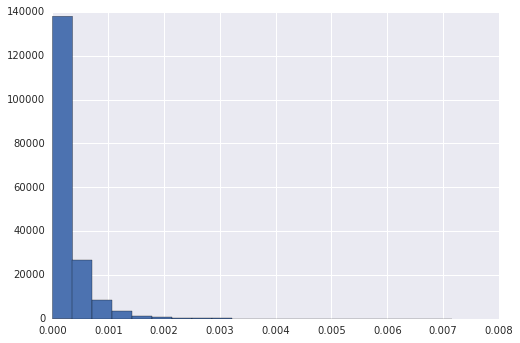
\includegraphics[width=45mm]{disp1.png} &   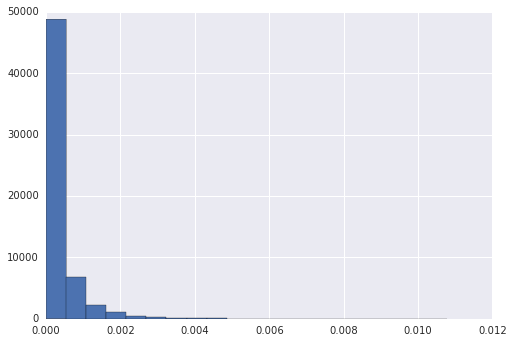
\includegraphics[width=45mm]{disp2.png} \\
 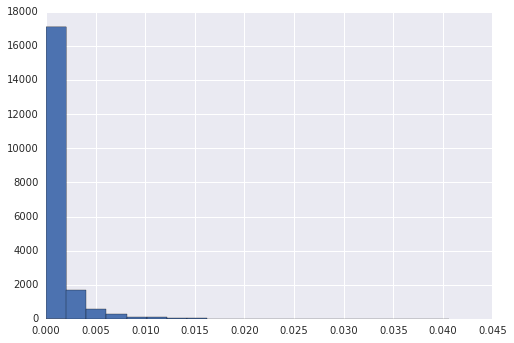
\includegraphics[width=45mm]{disp3.png} &   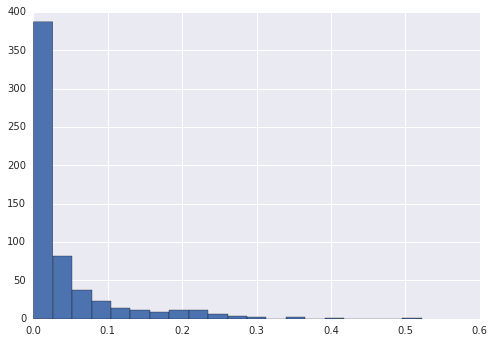
\includegraphics[width=45mm]{disp4.png} \\
\end{tabular}
}
\caption{Дисперсии параметров по слоям сети.}
\label{fig_disp}
\end{figure}
\end{frame}

\begin{frame}{Ковариационная матрица параметров}
\begin{figure}[h]
\noindent\centering{
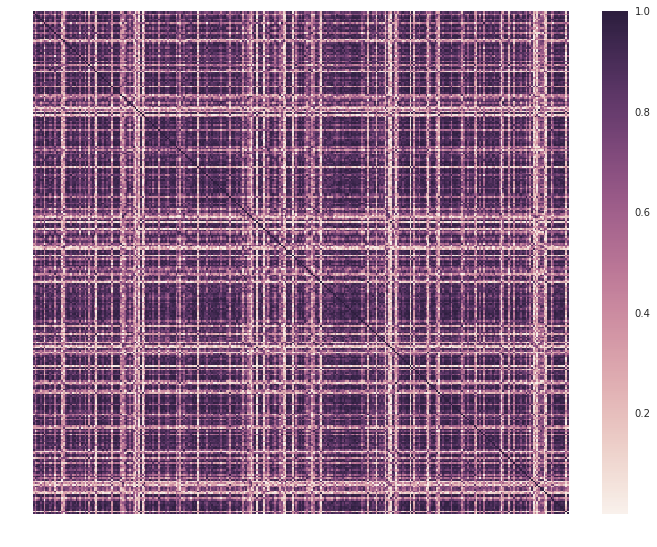
\includegraphics[width=80mm]{cov.png}
}
\caption{Ковариационная матрица весов нейрона.}
\label{fig_time_acc}
\end{figure}
\end{frame}


\begin{frame}{Результаты}
Исследовалась зависимость точности дообученной модели на тестовой выборке в зависимости от процента удалённых параметров при различных условиях выбора данных параметров.
\begin{figure}[h]
\noindent\centering{
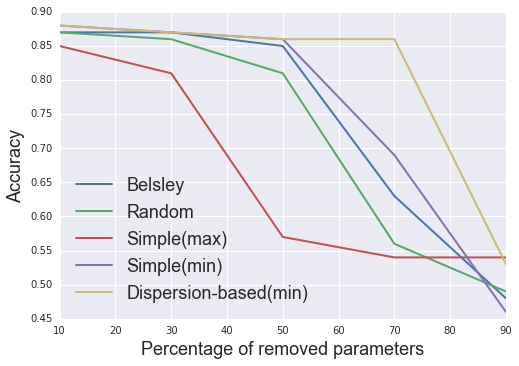
\includegraphics[width=70mm]{lines.png}
}
\caption{Зависимость точности модели от процента удалённых параметров.}
\label{fig_time_acc}
\end{figure}
\end{frame}

\begin{frame}{Заключение}
\begin{itemize}
\item Исследованы различные методы модификации пространства параметров модели в процессе обучения.
\item Получен эффективный метод разряжения сети глубокого обучения.
\end{itemize}
\end{frame}


\end{document}









